\everymath{\displaystyle}

\chapter{Ứng Dụng Mạng Nơ-ron Tích Chập Vào Bài Toán Nhận Diện Biển Báo Giao Thông }
\label{chap:chap5}

\section{Dữ liệu}
\subsection{Thông tin dữ liệu}
\hspace{5mm}Dữ liệu được sử dụng trong tài liệu này là German Traffic Sign Recognition Benchmark \cite{GTSRB} có hơn 50000 ảnh được chia ra 43 loại biển báo giao thông. 
\begin{figure}[H]
\begin{center}
\label{fig:data_sample}
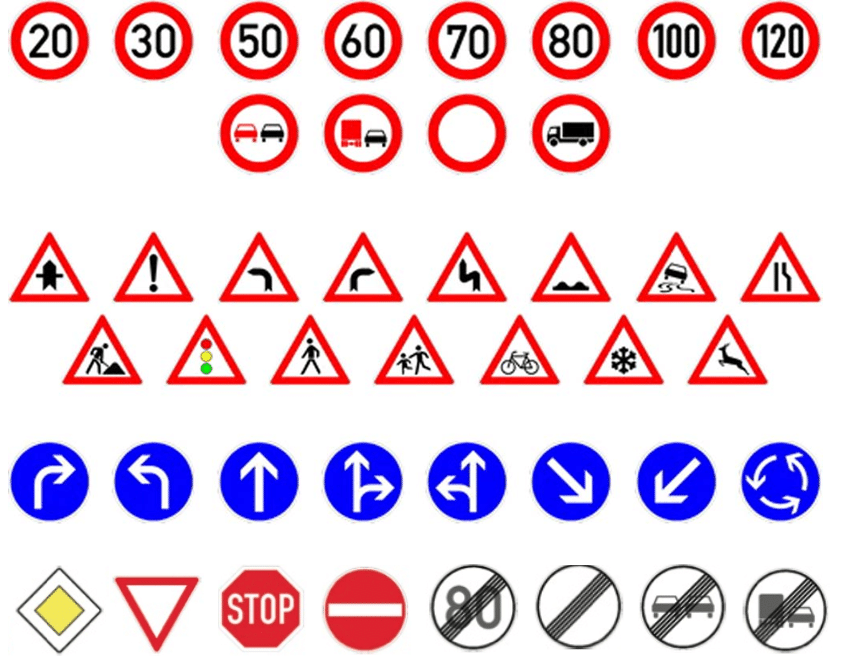
\includegraphics[scale=0.5]{chap5/image/data_sample.png}
\caption{Danh sách các loại biển báo}
\end{center}
\end{figure}
Trong 50000 ảnh biển báo giao thông, có gần 40000 ảnh được dùng trong quá trình huấn luyện, hơn 12000 dùng để kiểm tra và kích thước ảnh được trải từ $15\times 15$ đến $250\times250$ pixels và có định dạng file là '.ppm'. Biển báo ở lớp thứ 2 có nhiều số lượng nhiều nhất là 2250 ảnh, biển báo có lượng ít nhất ở lớp 0 với 210 ảnh.
\begin{figure}[H]
\begin{center}
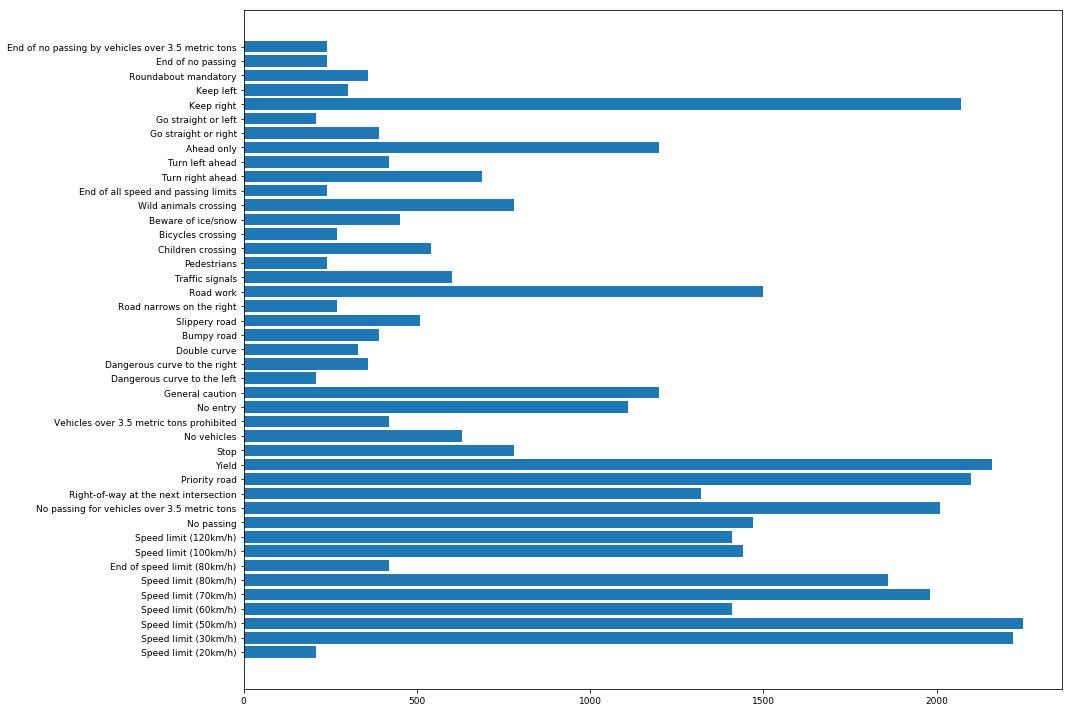
\includegraphics[scale=0.3]{chap5/image/data_statistic_ori.png}
\caption{Thống kê dữ liệu huấn luyện}
\label{fig:data_statistic}
\end{center}
\end{figure}
%\textbf{Tổ chức dữ liệu}\par
Dữ liệu được chia làm hai thư mục chính: thư mục chứa tập dữ liệu huấn luyện và thư mục chứa dữ liệu kiểm tra. Trong thư mục dữ liệu huấn luyện, dữ liệu được phân chia thành 43 thư mục con tương ứng với các loại biển báo và được đánh số id từ 0000 đến 0042, chi tiết tên và id được mô tả ở phần phục lục. Trong mỗi thư mục con là các ảnh của biển báo tương ứng và một file csv chứa tên đầy đủ của file ảnh và nhãn của nó. Trong thư mục dữ liệu kiểm tra sẽ là các dữ liệu không xuất hiện trong tập huấn luyện và một file lưu thông tin giống như ở trong tập huấn luyện.
\begin{figure}[H]
\begin{center}
\subfloat[Danh sách nhãn]
  {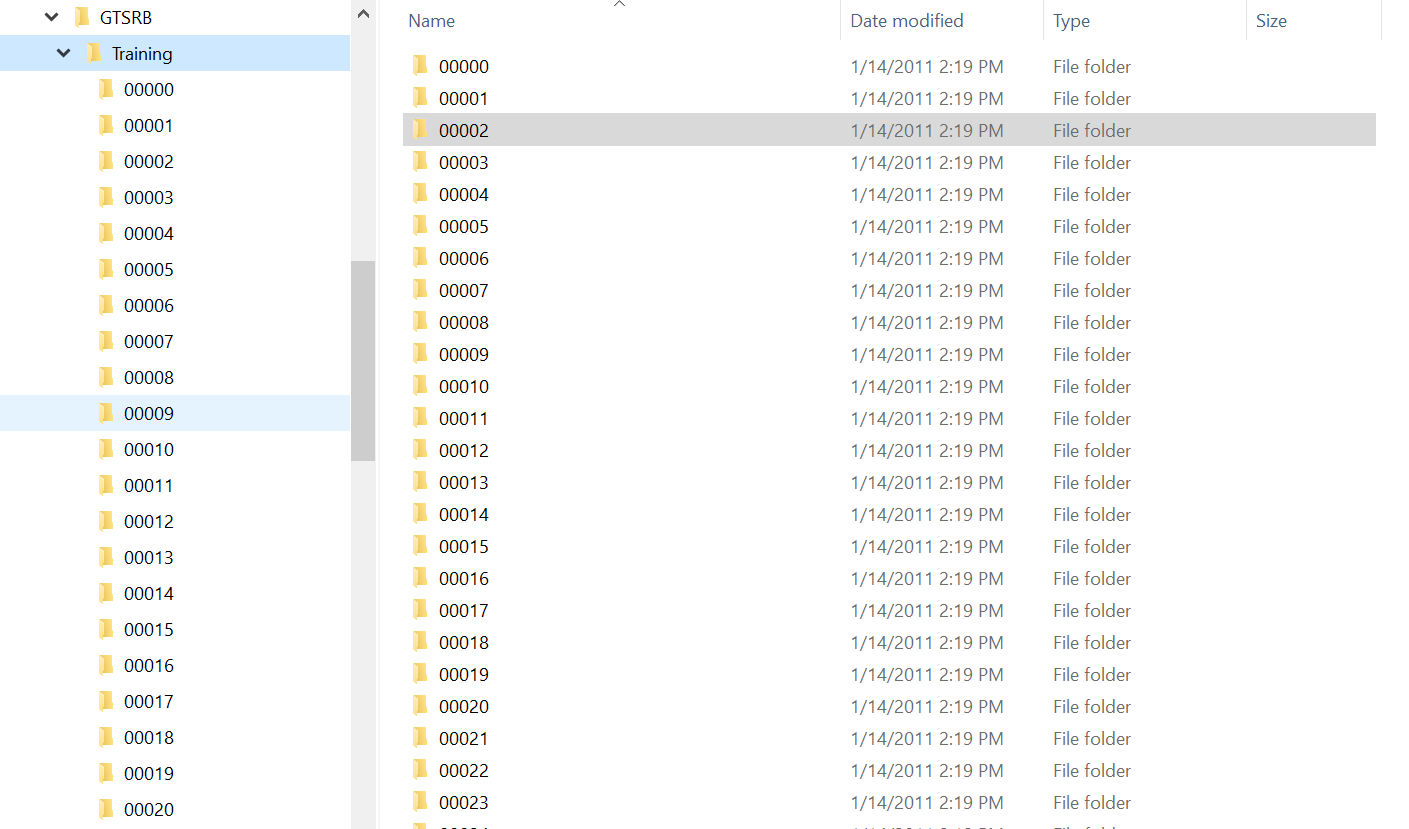
\includegraphics[width=.3\linewidth]{chap5/image/thumuc1.png}}\hspace{0.3cm}
\subfloat[Thư mục nhãn]
  {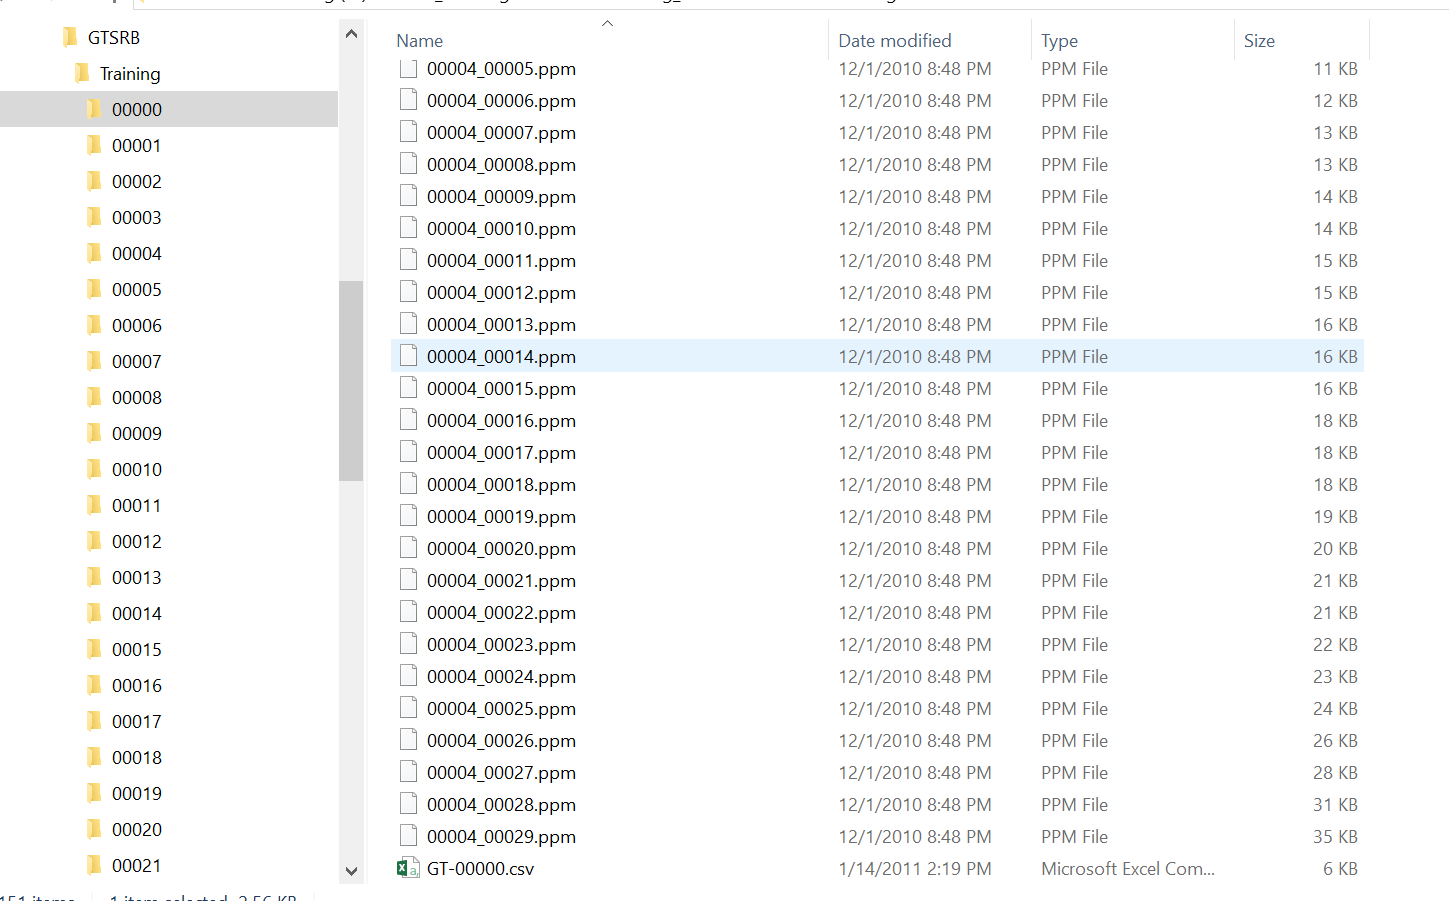
\includegraphics[width=.3\linewidth]{chap5/image/thumuc2.png}}
\subfloat[Thông tin dữ liệu của một nhãn]
  {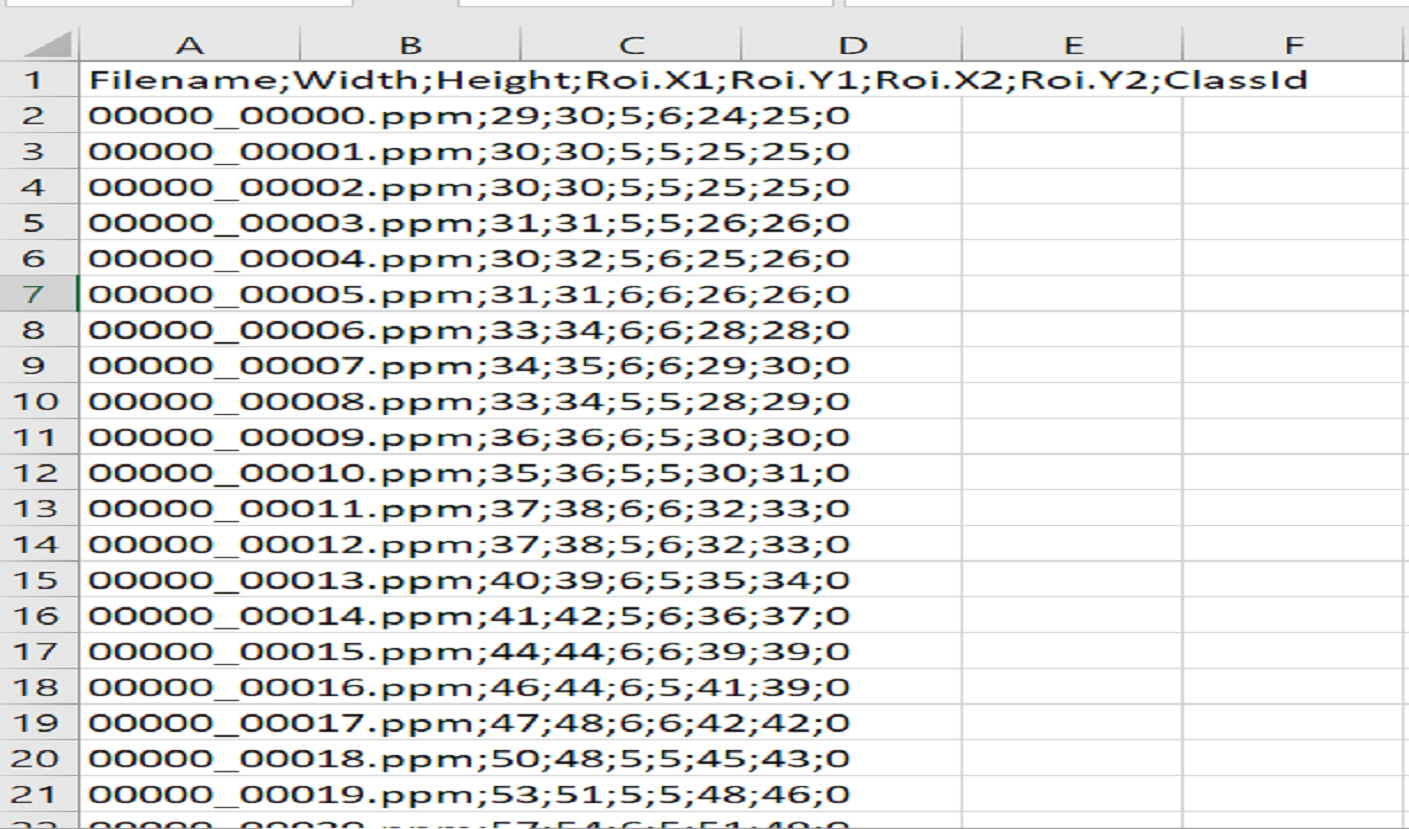
\includegraphics[width=.3\linewidth]{chap5/image/thumuc3.png}}
\caption{Cấu trúc thư mục}
\end{center}
\end{figure}
\subsection{Tăng cường dữ liệu}
\hspace{5mm} Dữ liệu sẽ được chia ra làm hai phần: phần sử dụng trong quá trình huấn luyện và phần sử dụng trong quá trình đánh giá. Trong đó phần đánh giá sẽ chiếm 25\% dữ liệu ban đầu. Sau khi chia dữ liệu dữ liệu huấn luyện được thống kê ở hình \ref{fig:train_split}, ta thấy dữ liệu không được phân chia đều ở các lớp, ở lớp 1 có dữ liệu nhiều nhất 1691 ảnh và lớp ít nhất chỉ có 147 ảnh là lớp 37. Vì thế để tạo cho cân bằng chúng ta sẽ tạo ra thêm dữ liệu từ dữ liệu ban đầu. Đối với các loại biển báo có ít mẫu dữ liệu, tôi sử dụng một số phương pháp như: xoay ảnh, phóng to, thu nhỏ, dịch chuyển,... sao cho số lượng mẫu giữa các loại biển báo tương đương nhau và 1.3 lần với lớp có số lượng mẫu dữ liệu lớn nhất.
Tổng số dữ liệu có được sau khi tăng cường là 89090 mẫu. Trong đó lớp có số lượng mẫu nhiều nhất là 31 có 2172 mẫu, lớp có số lượng mẫu ít nhất 3 có 1977 mẫu (hình \ref{fig:train_aug}). 

\begin{figure}[H]
\subfloat[Dữ liệu huấn luyện sau khi chia \label{fig:train_split}]
  {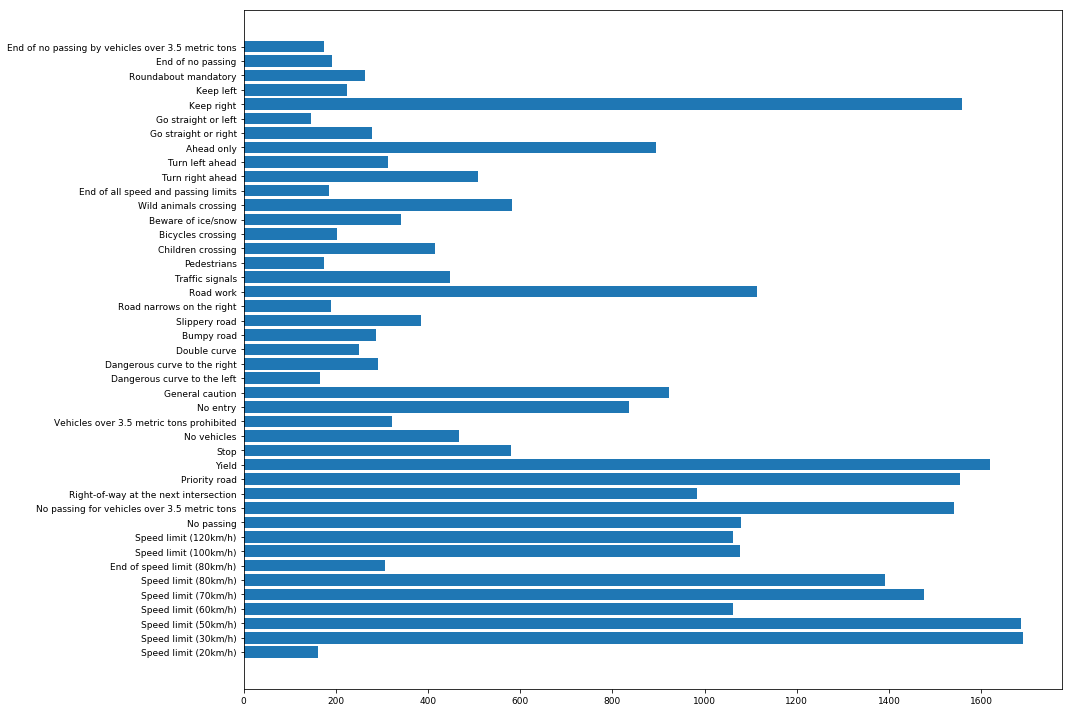
\includegraphics[width=.5\linewidth]{chap5/image/data_statistic.png}}\hspace{0.3cm}
\subfloat[Dữ liệu huấn luyện sau khi tăng cường \label{fig:train_aug}]
{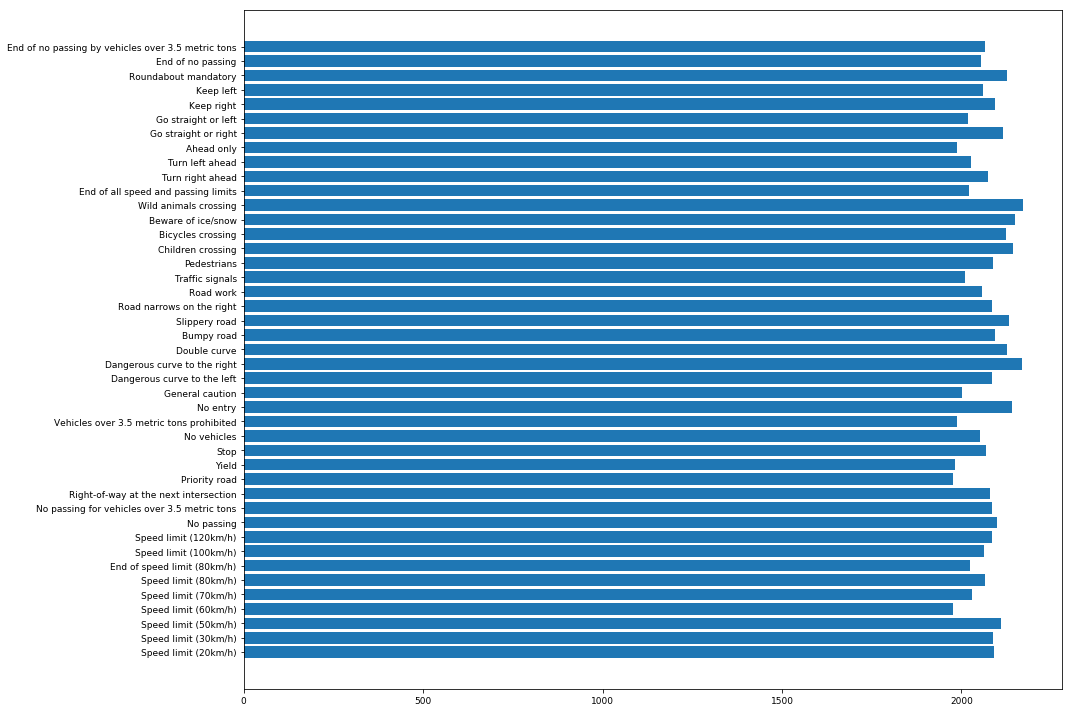
\includegraphics[width=.5\linewidth]{chap5/image/data_statistic2.png}}
\caption{Thống kê dữ liệu huấn luyện}
\end{figure}
Dưới đây là một số ảnh sau khi đã được áp dụng các phương pháp tăng cường dữ liệu.
\begin{figure}[H]
\subfloat[]
  {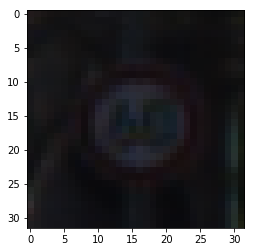
\includegraphics[width=.3\linewidth]{chap5/image/data_gen_ori_1.png}}\hspace{0.3cm}
\subfloat[]
  {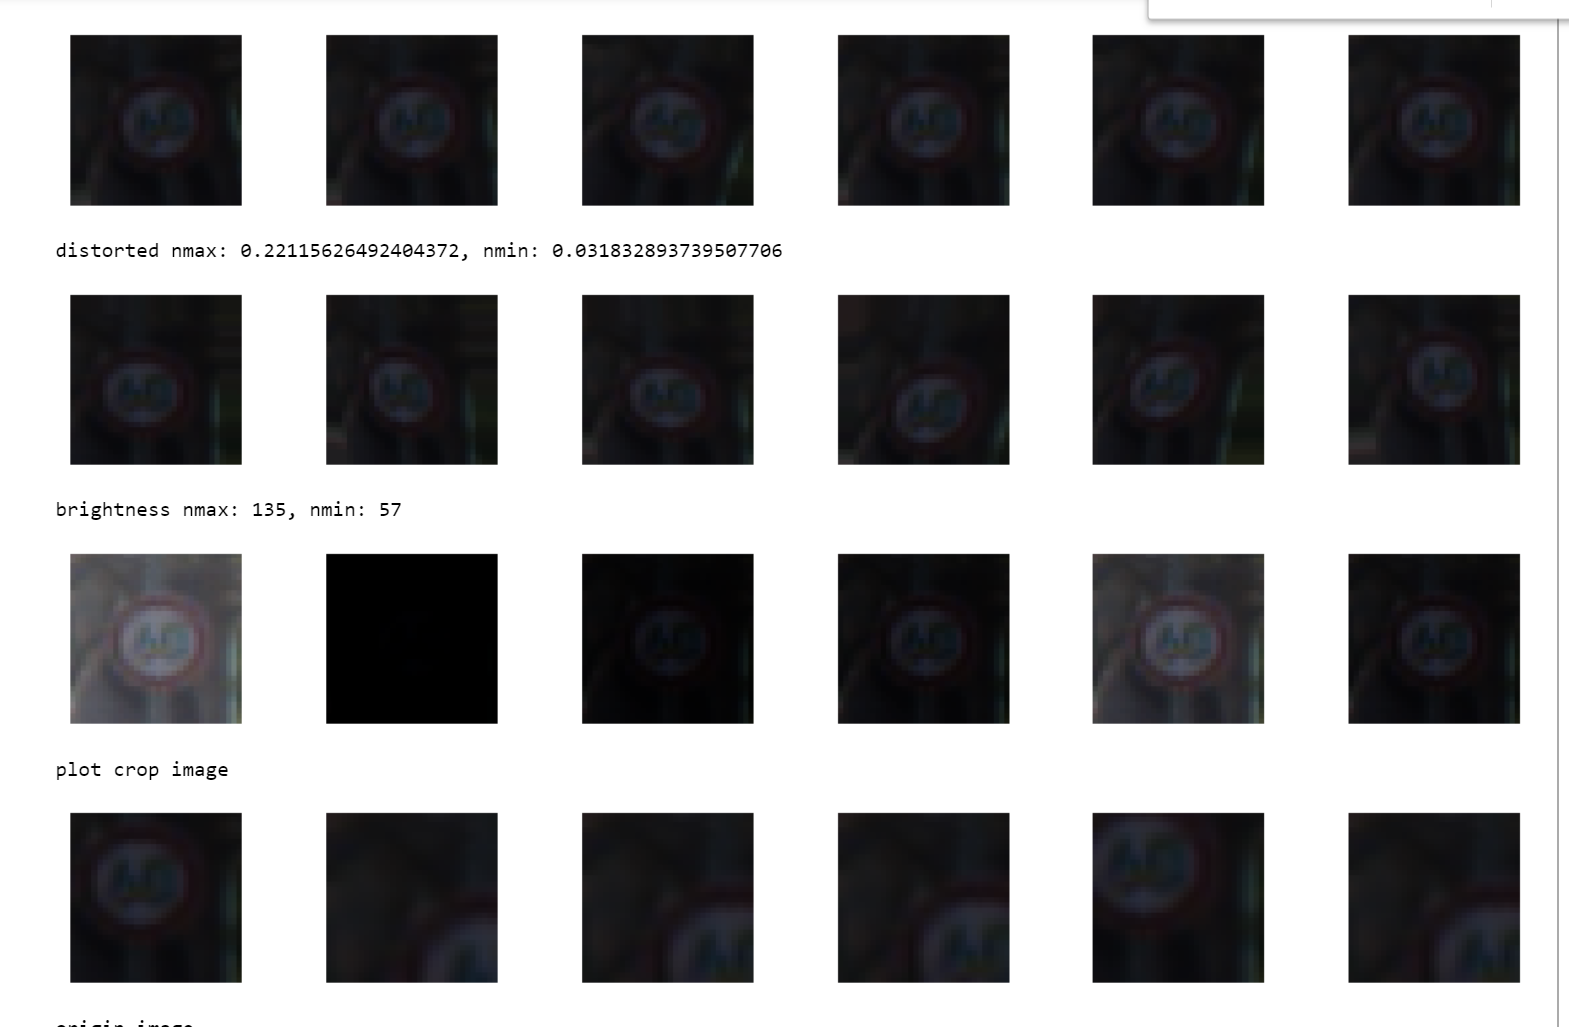
\includegraphics[width=.7\linewidth]{chap5/image/data_gen_1.png}}
\end{figure}
\begin{figure}[H]
\subfloat[]
  {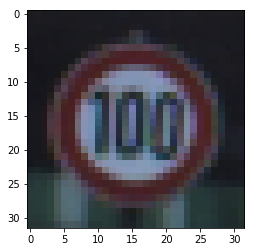
\includegraphics[width=.3\linewidth]{chap5/image/data_gen_ori_2.png}}\hspace{0.3cm}
\subfloat[]
  {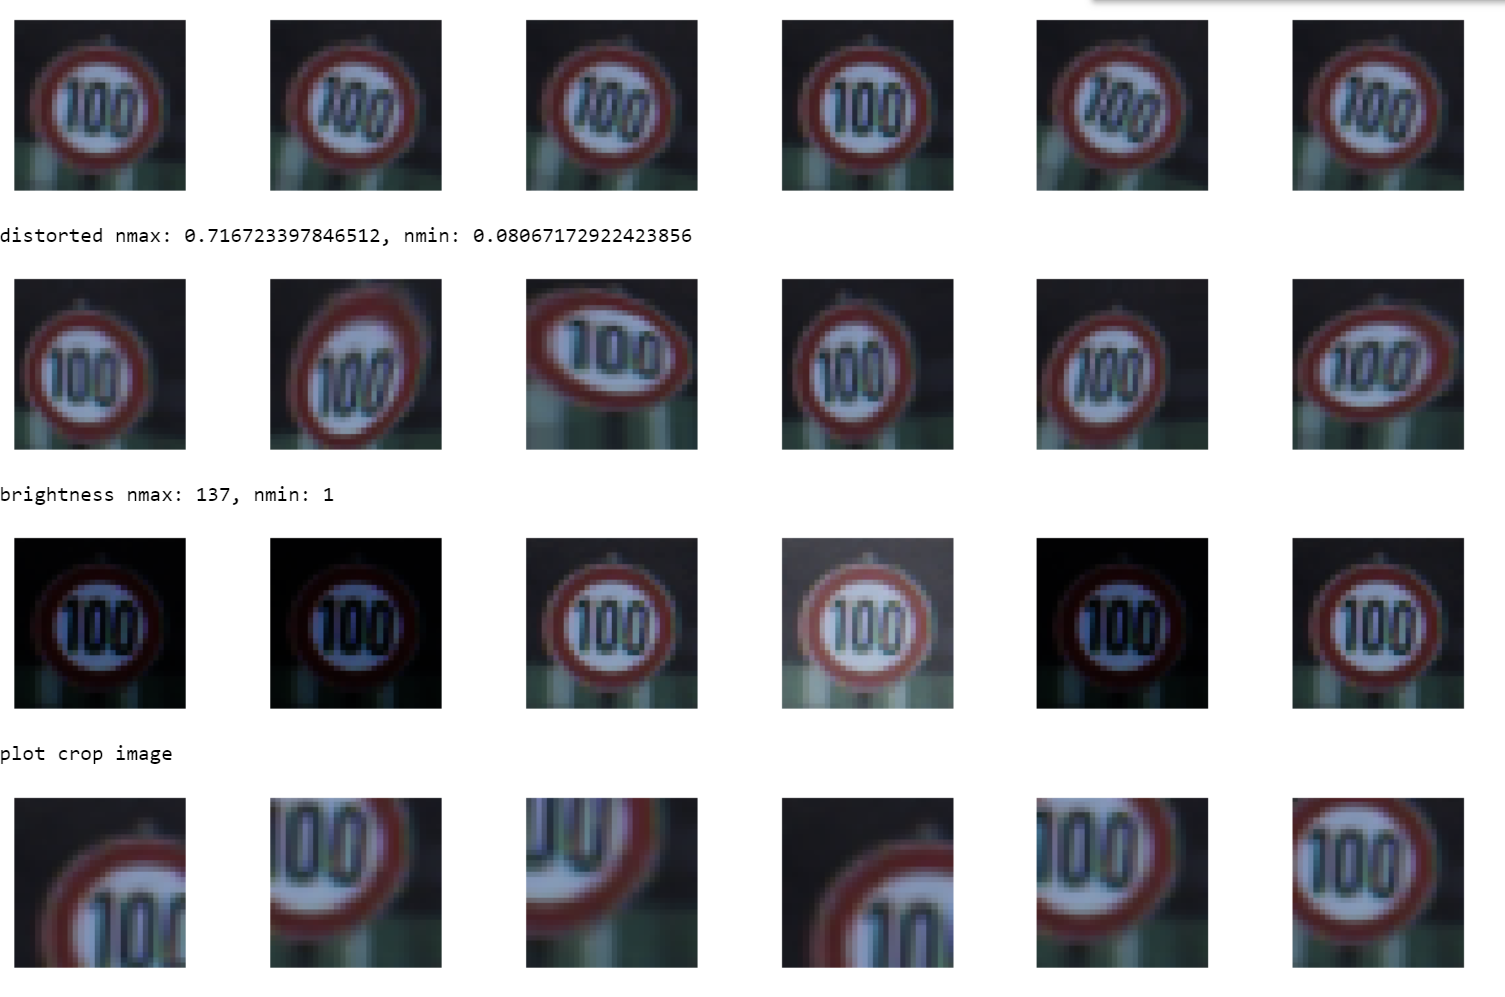
\includegraphics[width=.7\linewidth]{chap5/image/data_gen_2.png}}
\caption{Ảnh trước và sau khi tăng cường}
\end{figure}
\subsection{Chuẩn hóa dữ liệu}
Tất cả dữ liệu sẽ được chuyển về ảnh gray, mỗi giá trị điểm ảnh (Pixel) trong ma trận điểm ảnh mang giá trị từ 0 đến 255, chỉ có một chiều, kích thước là $32 \times 32$ pixels và các giá trị pixel co lại về trong khoảng giá trị $[0,1]$ để thuận tiện trong việc tính toán bằng cách lấy giá trị của mỗi pixel chia cho 255. Và tiếp theo đưa dữ liệu chúng ta về phân phối chuẩn với trung bình cộng $\mu$ và độ lệch chuẩn $\sigma$
\begin{align*}
\mu = \frac{1}{nwh}\sum_{k=1}^{n}\sum_{j=1}^{w}\sum_{i=1}^{h}pixel_{ij}^{(k)};\hspace{5mm}
\sigma = \sqrt{\frac{1}{nwh}\sum_{k=1}^{n}\sum_{j=1}^{w}\sum_{i=1}^{h}(pixel_{ij}^{(k)} - mean)^2}\\
\textit{trong đó $n$ là số lượng dữ liệu kiểm tra, $w,h$ là chiều rộng và chiều cao của mỗi ảnh}
\end{align*}
Sau khi có được $\mu$ và $\sigma$ thì dữ liệu được chuẩn hóa dữ liệu bằng cách:
\begin{align*}
pixel^{(k)} = (pixel^{(k)} - \mu)/\sigma
\end{align*}
Dưới đây là một số hình ảnh trong tập huấn luyện đã được chuẩn hóa.
\begin{figure}[H]
\begin{center}
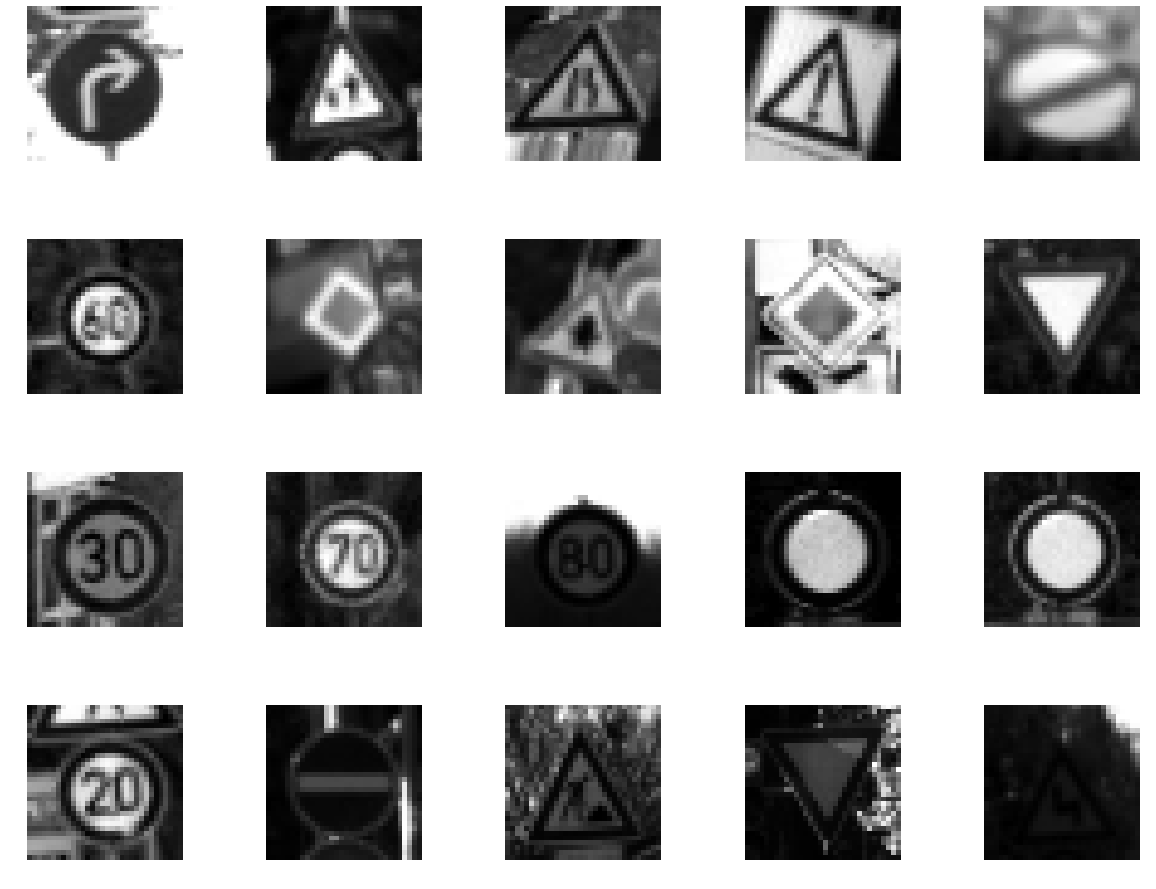
\includegraphics[width=.7\linewidth]{chap5/image/data_gray.png}
\caption{Dữ liệu đã được chuẩn hóa}
\end{center}
\end{figure}

\section{Xây dựng mô hình}
Tôi sẽ xây dựng 2 mô hình, một mô hình gồm 8 tầng và được xây dựng từ đầu, mô hình còn lại là sử dụng mạng VGG16 (mục \ref{sec:vgg16}) làm pretrain \footnote{Model đã được huấn luyện với lượng lớn dữ liệu, có khả năng trích xuất được đa dạng các đặc tính của ảnh. Sử dụng đúng pre-trained có thể giúp model cải tiến thêm nhưng không phải lúc nào cũng như vậy.} để trích xuất đặc trưng. Kết quả sẽ được so sánh ở phần đánh giá mô hình.
\subsection{Mô hình 11 tầng}
\label{sec:model1}
Mô hình này được xây dưng bao gồm: 6 tầng tích chập, 3 tầng giảm số chiều và fully-connected có 2 tầng. Trong đó 9 tầng đầu tiên được chia làm 3 phần giống nhau: 2 tầng tích chập trước, một tầng giảm số chiều đằng sau, đầu ra của tầng giảm số chiều ở phần trước làm đầu vào cho tầng tích chập đầu tiên ở phần sau. Đầu vào ở tầng thứ 10 sẽ là một vector 1 chiều được làm "phẳng" bởi tầng giảm số chiều cuối cùng. Và tầng cuối cùng là tầng fully-connected, quyết định dữ liệu thuộc nhãn nào. \par
Tại các tầng tích chập, bộ lọc có kích thước là $3x3$, bước trượt bằng 1, hàm kích hoạt là relu và đầu ra có kích thước bằng với đầu vào. Số lượng bộ lọc mỗi tầng lần lượt là 32, 32, 64, 64, 128, 128. Ở tầng giảm số chiều, ta lựa chọn theo pixel có giá trị lớn nhất với bộ lọc là $2x2$ và bước trượt là 2. Tại tầng fully-connected, với đầu vào là đầu ra của lớp giảm số chiều cuối cùng được làm phẳng và dropout bằng $0.2$. Kiến trúc được xây dựng gồm một tầng với số lượng nơ-ron là 512 và một tầng có kích thước là 43 tương ứng với số lượng lớp cần phân loại. Ta sử dụng softmax làm hàm kích hoạt cho lớp cuối cùng và relu cho tầng trước đó. Tổng số lượng các trọng số của mô hình ta cần tính toán là 898827. Mô hình được huấn luyện với 30 epochs\footnote{epoch là một lần chạy lan truyền thẳng và lan truyền ngược cho tất cả dữ liệu huấn luyện}, trong khoảng 15 phút.
\begin{figure}[H]
\begin{center}
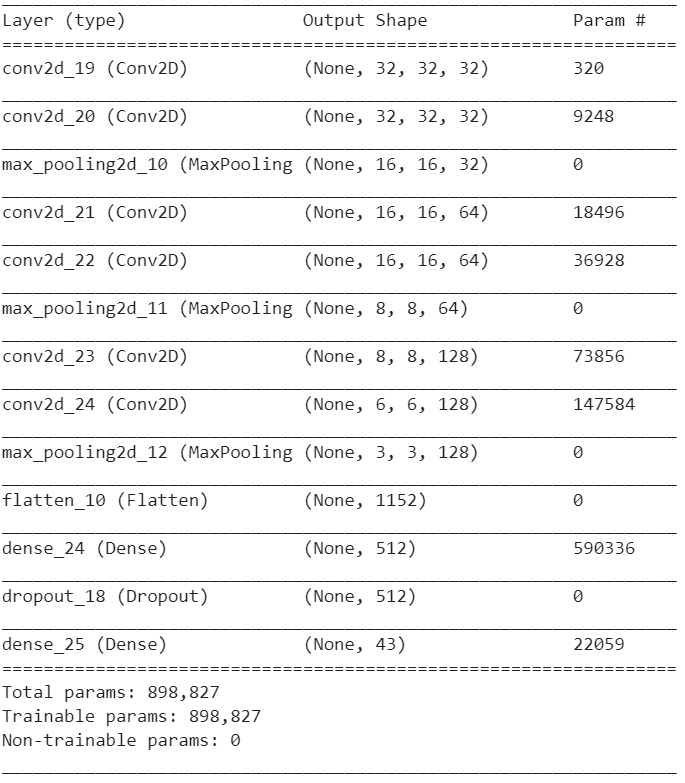
\includegraphics[scale=1]{chap5/image/model/model_endtoend.png}
\end{center}
\caption{Mô hình 11 tầng}
\end{figure}
\subsection{Mô hình sử dụng pre-trained}
Ta sẽ xây dựng mô hình với phần trích xuất đặc trưng là mô hình VGG16 và phần phân loại lớp hay tầng fully-connected sẽ được xây dựng tương tự với mô hình 11 tầng (\ref{sec:model1}) với 2 tầng nơ-ron có số lượng là 512 và 43. Mô hình VGG16 sẽ được giữ nguyên trọng số ở các block1, block2, block3, block4 còn block5 sẽ bị thay đổi trọng số. Đầu ra ở tầng cuối cùng của mô hình sẽ được làm phẳng và làm đầu vào cho tầng fully-connected. Tổng số lượng trọng số ở mô hình VGG16 là 14714688, trong đó có 7635264 trọng số được giữ nguyên và 7079424 trọng số bị thay đổi ở block5. Tổng số lượng trọng số ở mô hình với VGG16 làm pre-trained là 14999403, với số lượng trọng số không thay đổi bằng với mô hình VGG16 và số lượng trọng số cần tính sẽ tăng lên 7364139.
\begin{figure}[H]
\subfloat[Mô hình VGG16]
  {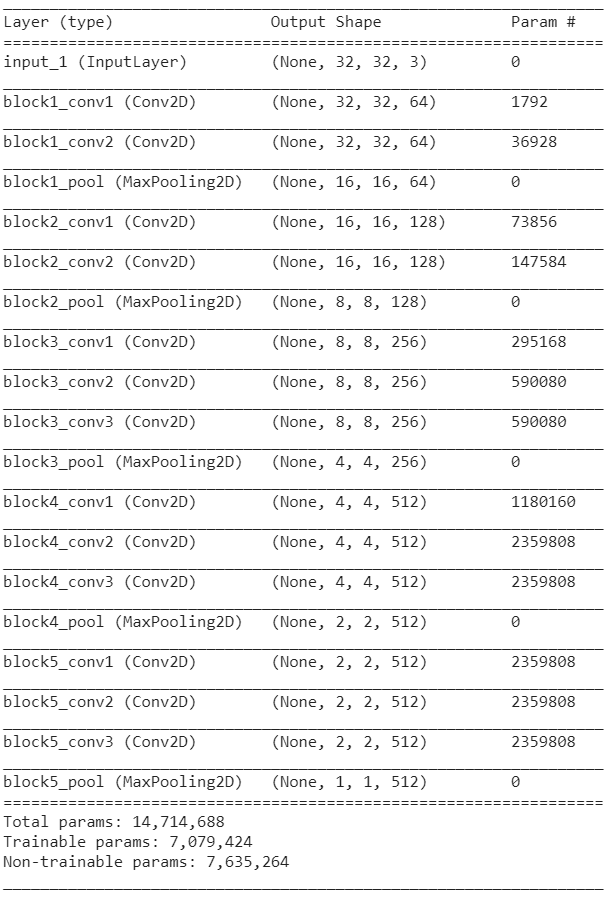
\includegraphics[width=.5\linewidth]{chap5/image/model/vgg16.png}}\hspace{0.3cm}
\subfloat[Mô hình với VGG16 làm pre-trained]
  {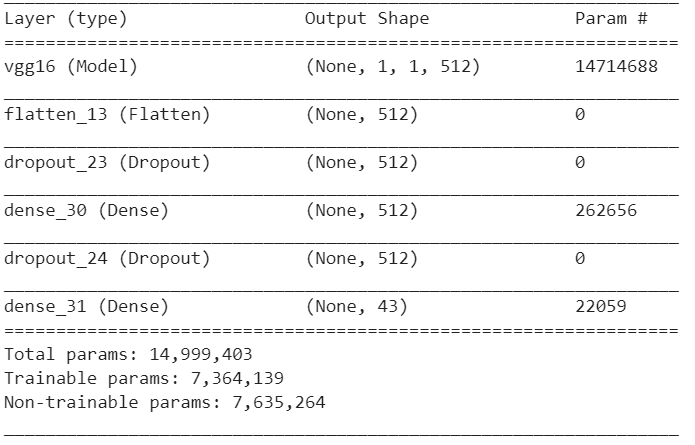
\includegraphics[width=.5\linewidth]{chap5/image/model/vgg16_with_my_layer.png}}
\caption{Mô hình VGG16 và mô hình sử dụng VGG16 làm pre-trained}
\end{figure}
\subsection{Đánh giá mô hình}
Như tôi đã trình bày, sử dụng pre-trained sẽ rất tốt, giúp chúng ta khắc phuc về cơ sở hạ tầng khi không đáp ứng được, giảm thời gian tính toán do không cần phải huấn luyện mô hình mà thay vào đó sử dụng các trọng số đã được tính trước. Và nó còn làm cơ sở để phát triển cho nhiều bài toán khác nhau. Tuy nhiên để chọn mô hình nào làm pre-trained thì chúng ta cần phải thử nhiều với các mô hình khác nhau hoặc kết hợp chúng lại với nhau để cho ra mô hình phù hợp với bài toán của chúng ta hơn.
\begin{figure}[H]
\subfloat[Mô hình 11 tầng \label{fig:result_model1}]
  {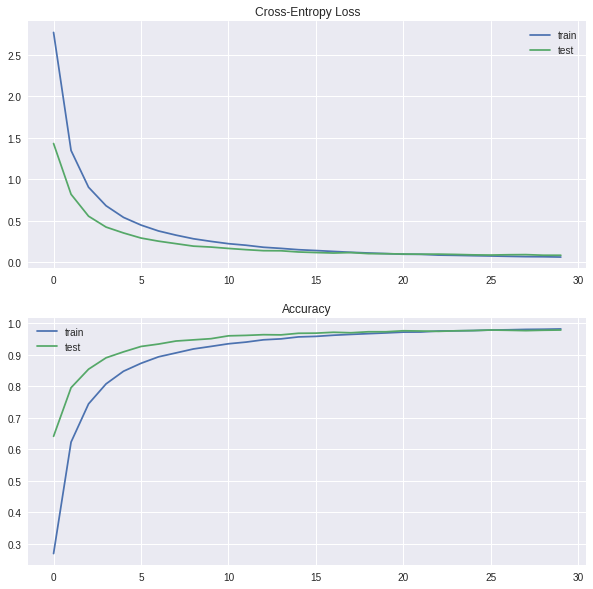
\includegraphics[width=.5 \linewidth]{chap5/image/model/result/ete.png}}\hspace{0.3cm}
\subfloat[Mô hình với VGG16 làm pretrain \label{fig:result_model2}]
  {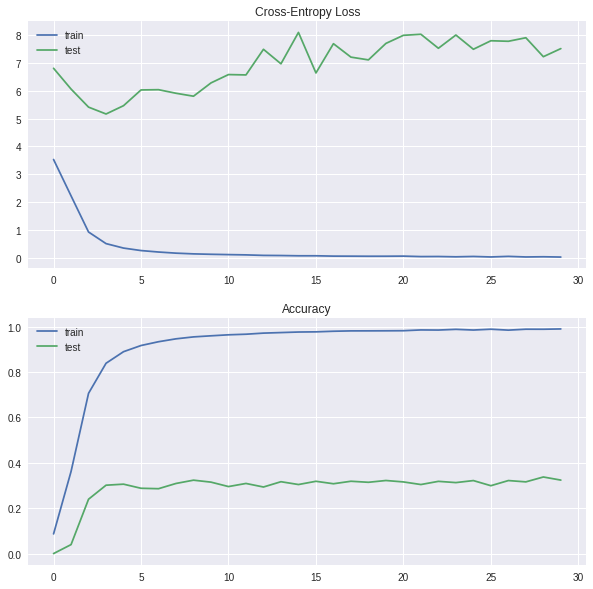
\includegraphics[width=.5\linewidth]{chap5/image/model/result/vgg.png}}
\caption{Biểu đồ mô tả giá trị mất, độ chính xác trong quá trình huấn luyện}
\end{figure}
Chúng ta có thể thấy rằng với kết quả của mô hình 11 tầng (hình \ref{fig:result_model1}) tốt hơn hẳn so với mô hình sử dụng VGG16 làm pretrain (hình \ref{fig:result_model2}). Ở mô hình 11 tầng giá trị mất mát được giảm theo thời gian và tiến gần đến 0, độ chính xác thì tiến dần đến 1. Còn ở mô hình với VGG16 làm pretrain thì giá trị mất mát trên tập huấn luyện giảm đi theo thời gian tiến gần đến 0 nhưng với tập validate thì không được giảm mà chỉ dao động trong khoảng từ 0.8 về đến 0.5. Với độ chính xác thì cũng tương tự, trên tập huấn luyện độ chính xác tiến gần đến 1 còn trên tập validate thì chỉ là 0.3. Như vậy chúng ta có thể kết luận rằng mô hình với VGG16 làm pretrain bị overfitting. \par
Trên tập kiểm tra,kết quả thu được của mô hình 11 tầng là: 95\%, còn trên mô hình với VGG16 làm pretrain là: 75\%. Chúng ta có thể thấy rõ hơn khi nhìn vào ma trận nhầm lẫn của từng mô hình.
\begin{figure}[H]
\begin{center}
\subfloat[Mô hình 11 tầng \label{fig:result_cm_model1}]
  {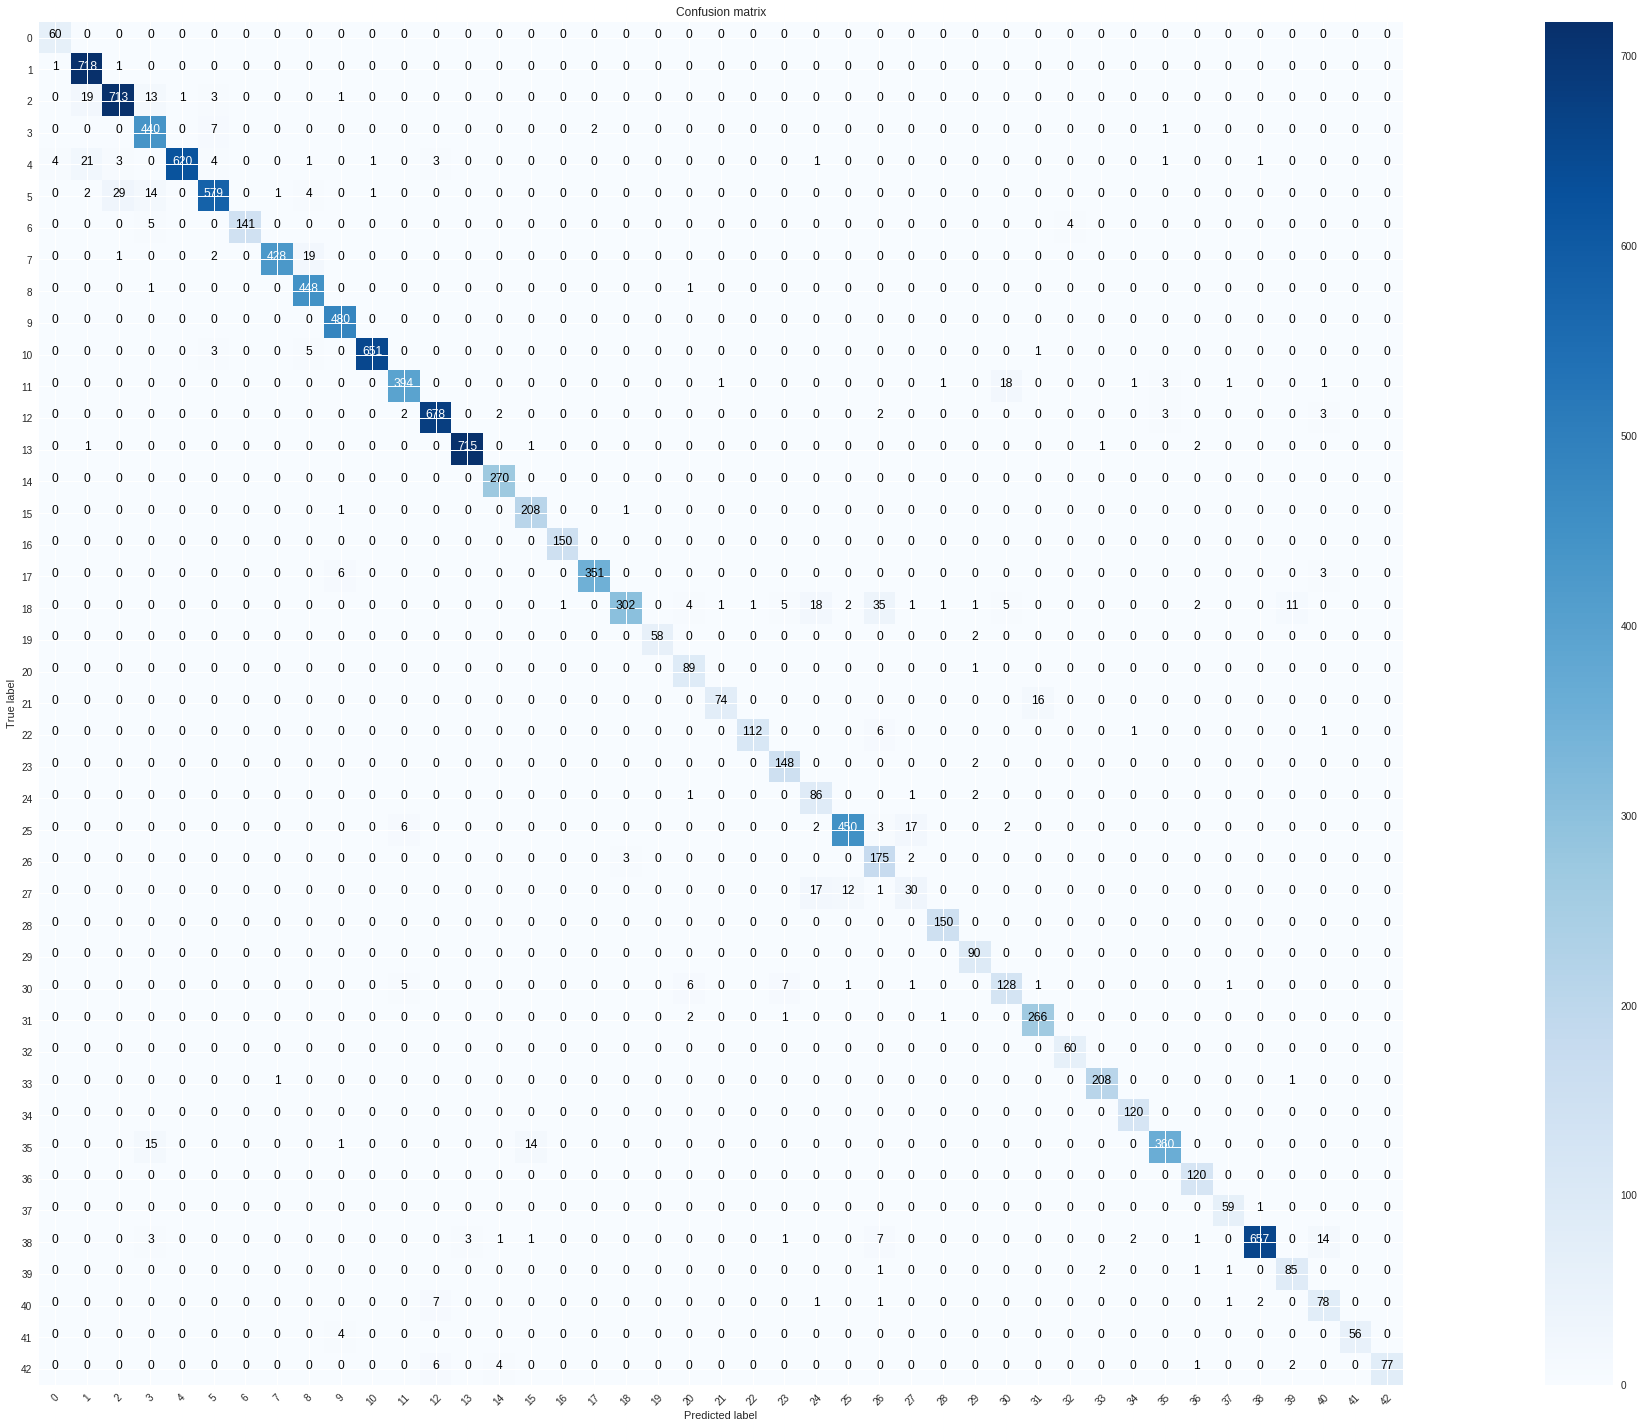
\includegraphics[width=.8\linewidth]{chap5/image/model/result/ete_matrix.png}}\hspace{0.3cm}
\subfloat[Mô hình với VGG16 làm pretrain \label{fig:result_cm_model2}]
  {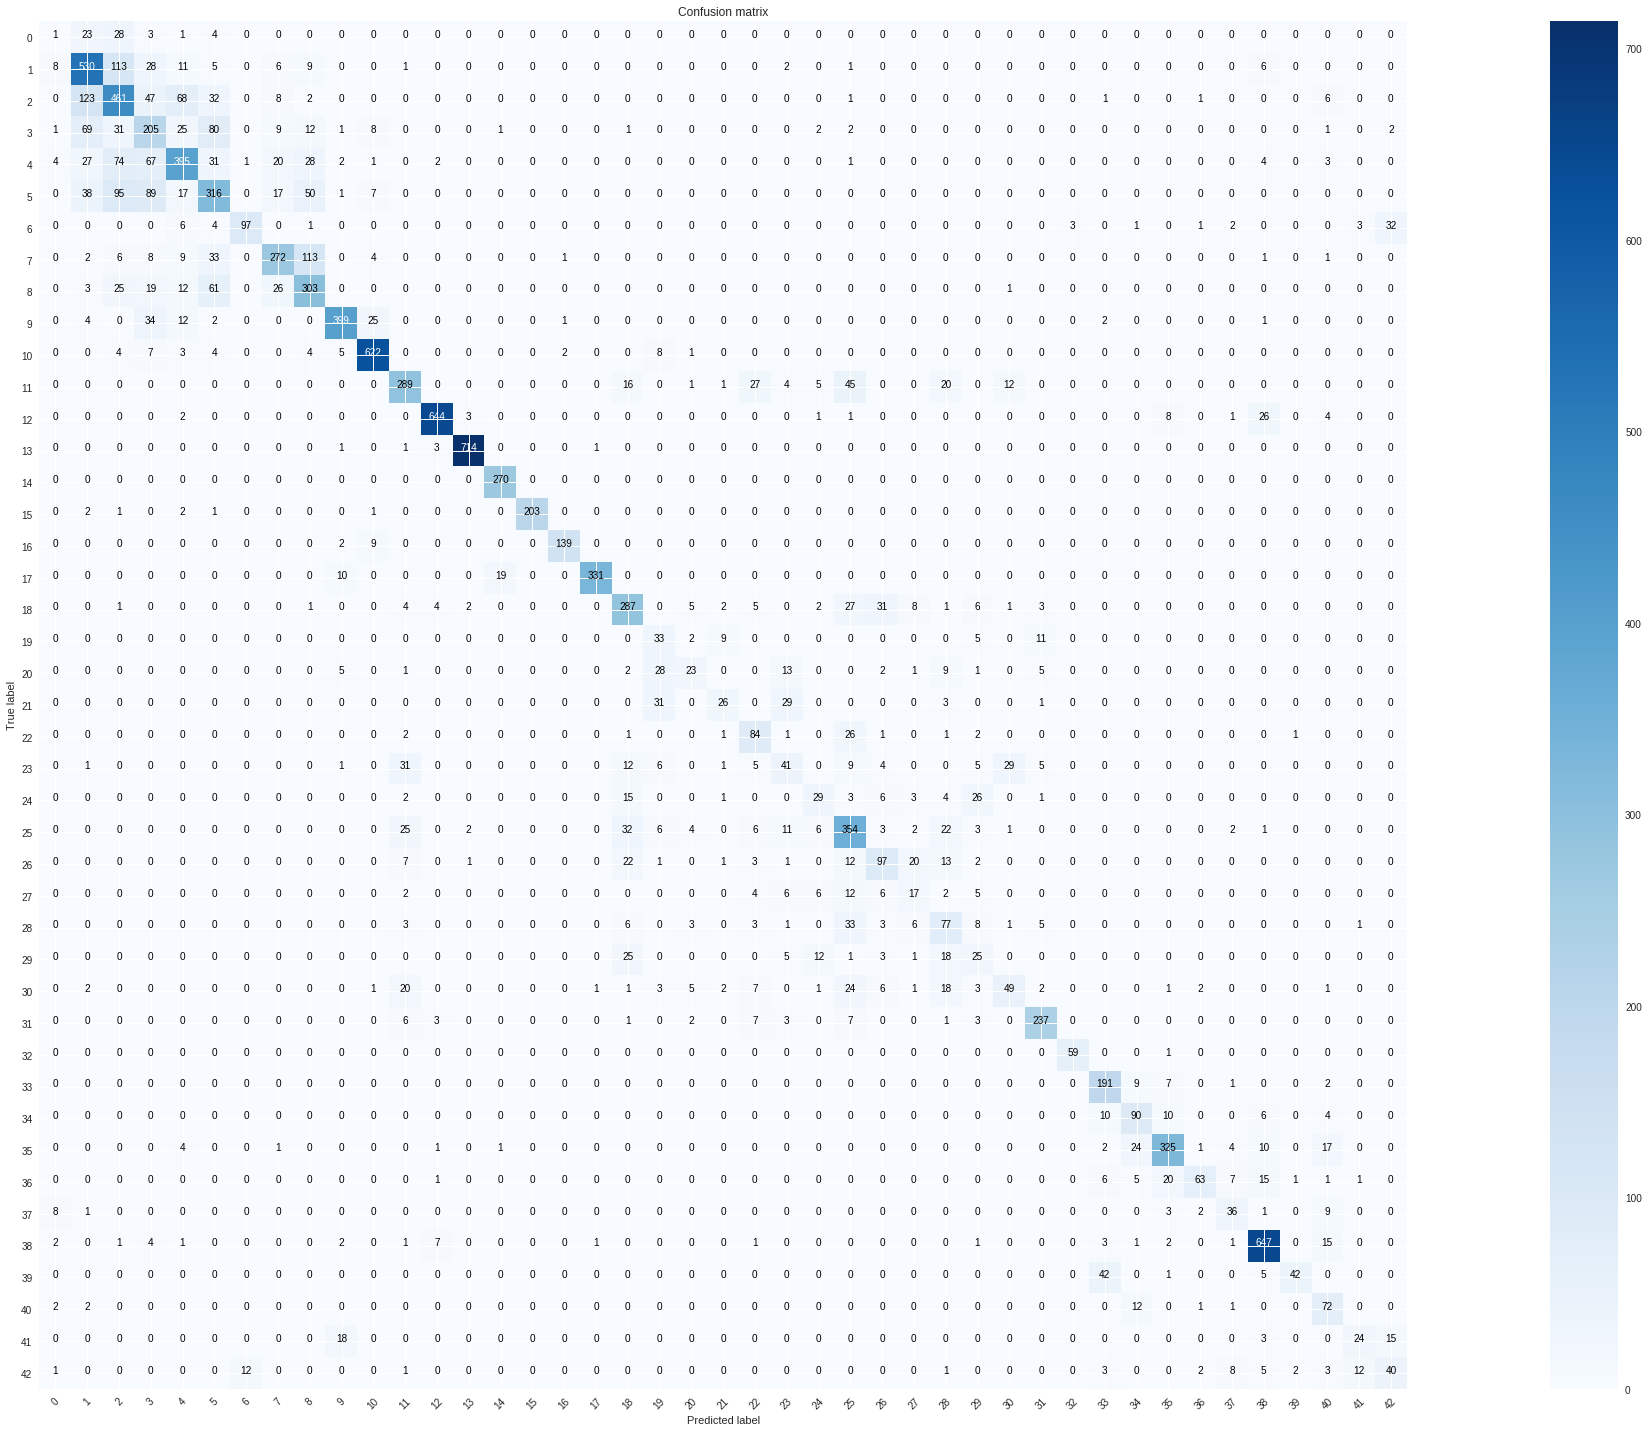
\includegraphics[width=.8\linewidth]{chap5/image/model/result/vgg_matrixx.png}}
\end{center}
\caption{Ma trận nhầm lẫn cho các mô hình}
\end{figure}
Hình \ref{fig:result_cm_model1} cho ta thấy tại lớp 0 có 60 ảnh thử nghiệm và không có ảnh nào bị dự đoán sai. Với lớp số 1 chúng ta có 720 đầu vào, dự đoán đúng là 718, có 2 ảnh bị dự đoán sai thành  lớp số 0 và lớp số 2. Tương tự với hình \ref{fig:result_cm_model2} ta có thể thấy ngay ở lớp số 0, tỉ lệ dự đoán đúng chỉ là $\frac{1}{60}$, còn dự đoán nhầm sang lớp số 1, lớp số 2, mỗi lớp 28 ảnh và lớp số 3,4,5 lần lượt là 3,1,4.
\section{Nhận diện biển báo giao thông}
Thuật toán được sử dụng cho bài toán nhận diện biển báo giao thông là YOLOv2. Mô hình sẽ được huấn luyện bằng thư viện drakflow \cite{drakflow}, là thư viện sử dụng mã nguồn mở darknet\cite{darknet13} để thực hiện thuật toán YOlOv2.\par
Dữ liệu là các ảnh toàn cảnh, trong đó chứa các biển báo giao thông và được định sẵn các bounding boxes cho biển báo.
\begin{figure}[H]
\centering
\subfloat[]
{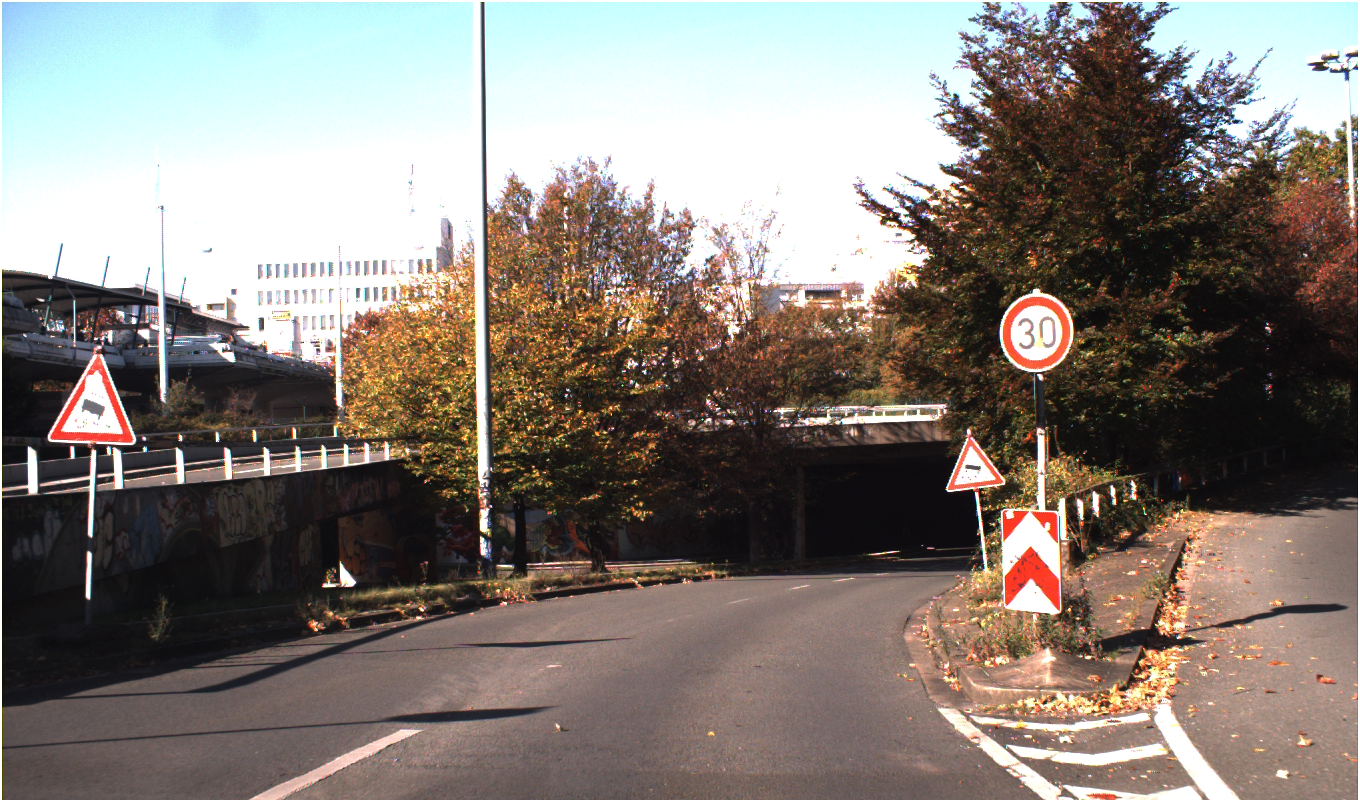
\includegraphics[scale=0.15]{chap5/image/data_detect/0.png}} \hspace{3mm}
\subfloat[]
{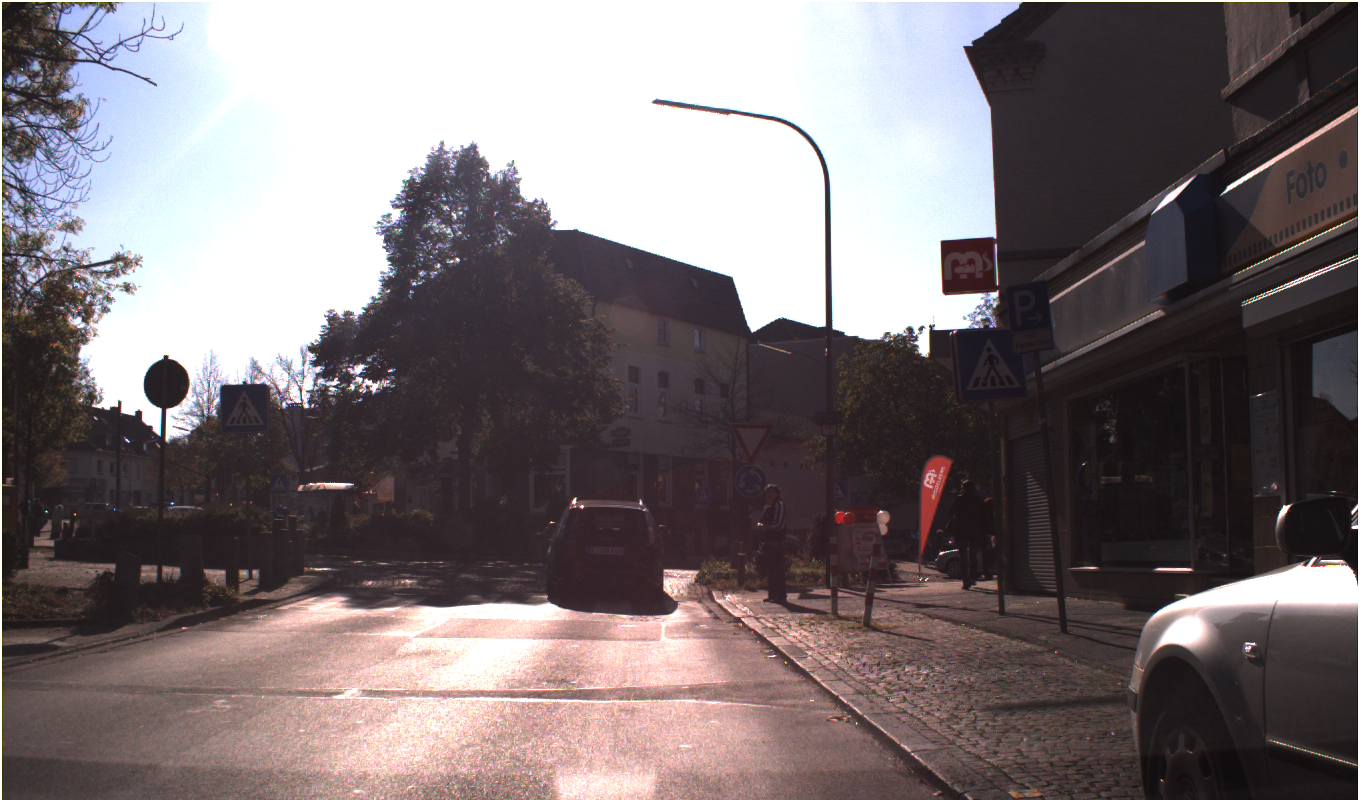
\includegraphics[scale=0.15]{chap5/image/data_detect/1.png}}\\
\subfloat[]
{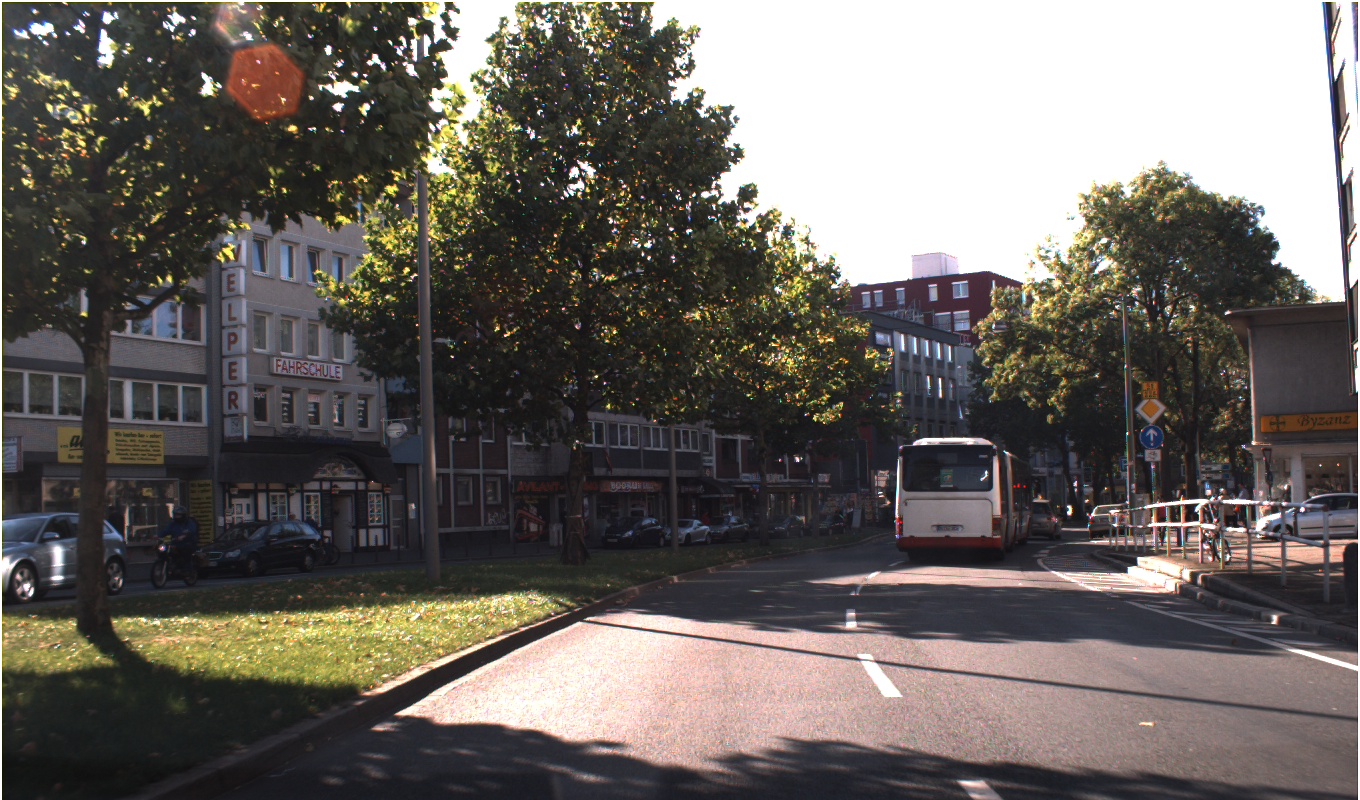
\includegraphics[scale=0.15]{chap5/image/data_detect/2.png}} \hspace{3mm}
\subfloat[]
{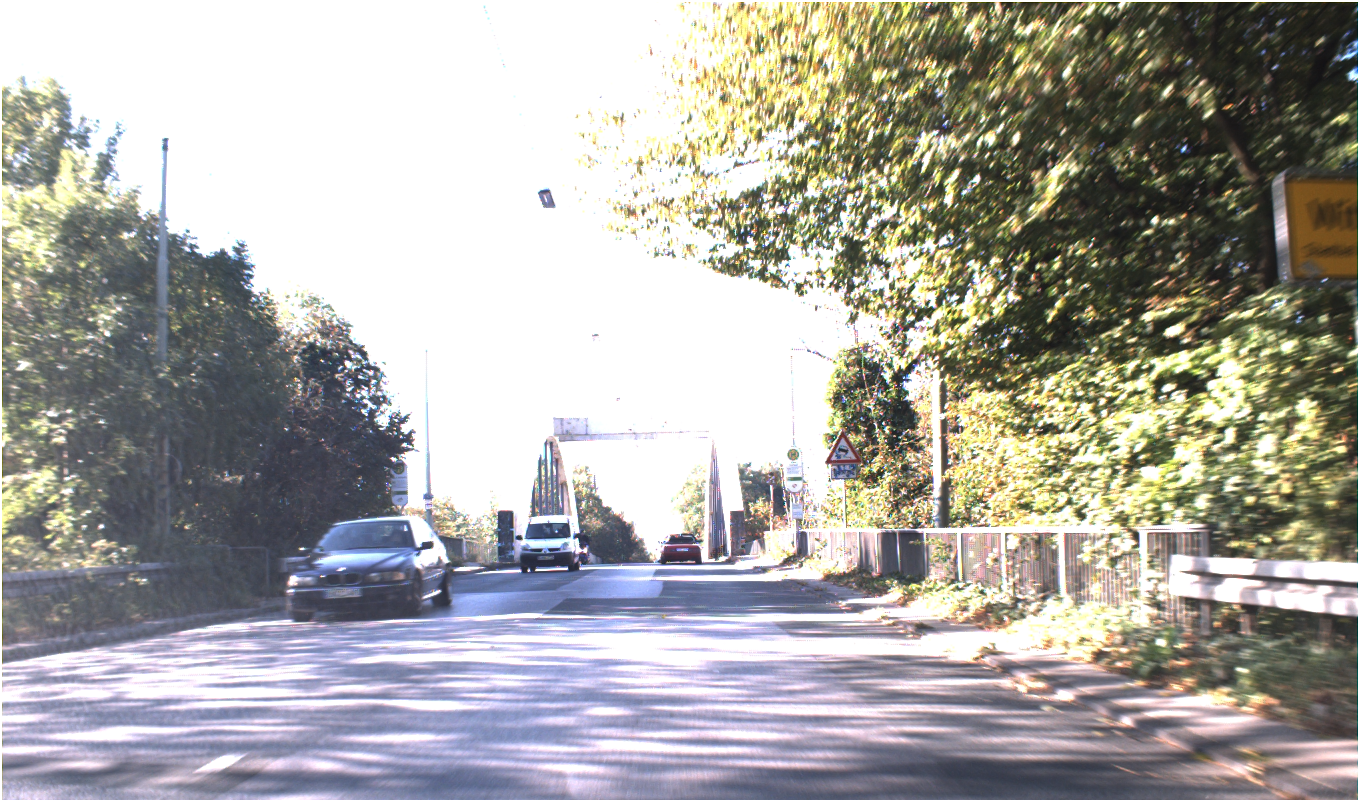
\includegraphics[scale=0.15]{chap5/image/data_detect/3.png}}
\caption{Một số hình ảnh trong dữ liệu huấn luyện}
\end{figure}
Các thông số vị trí biển báo được lưu vào file với tên là annotation.txt, ví dụ:
\begin{center}
00001.ppm;983;388;1024;432;0\\
00001.ppm;386;494;442;552;38
\end{center}
\hspace{5mm} Ý nghĩa:
\begin{center}
<tên ảnh><4 tọa đô xác định biển báo><id biển báo>
\end{center}
Các thông số này sẽ được chuyển đổi để phù hợp với đầu vào của drakflow theo định dạng dưới đây.
\begin{figure}[H]
\begin{center}
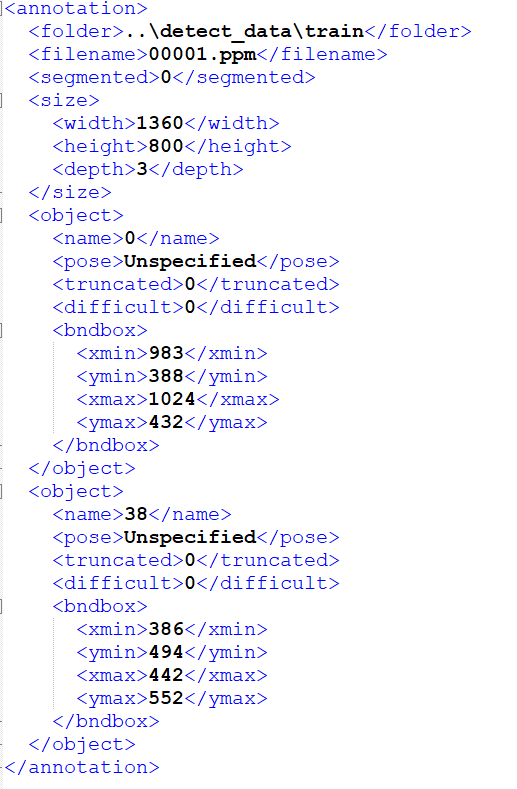
\includegraphics[scale=0.8]{chap5/image/annotation.png}
\end{center}
\caption{Đầu vào cho darknet}
\end{figure}
Dưới đây là một số hình ảnh được kiểm tra sau quá trình huấn luyện:
\begin{figure}[H]
 \centering
    \subfloat[]
     {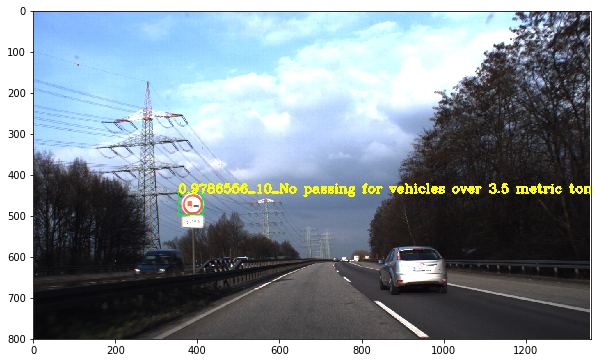
\includegraphics[height=2in]{chap5/image/data_detect/result/d3.png}}
    \subfloat[]
     {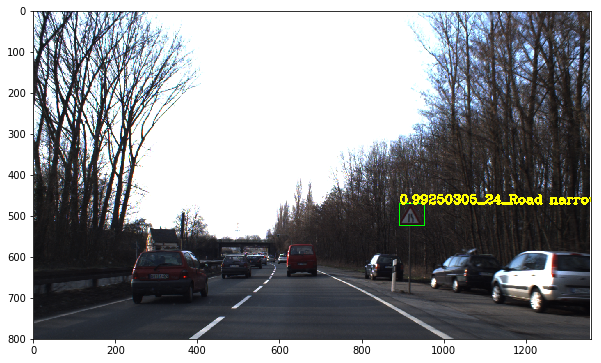
\includegraphics[height=2in]{chap5/image/data_detect/result/d4.png}}
\end{figure}
\begin{figure}[H]
     {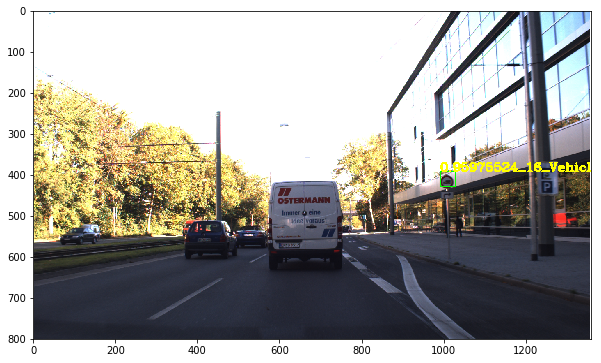
\includegraphics[height=2in]{chap5/image/data_detect/result/d6.png}}
    \subfloat[]
     {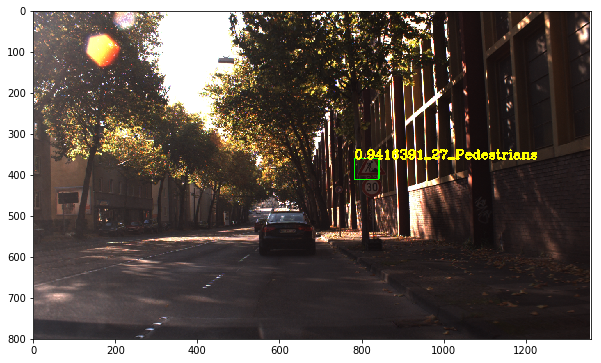
\includegraphics[height=2in]{chap5/image/data_detect/result/d7.png}}
\caption{Kết quả nhận diện đúng}
\end{figure}

\begin{figure}[H]
 \centering
    \subfloat[]
     {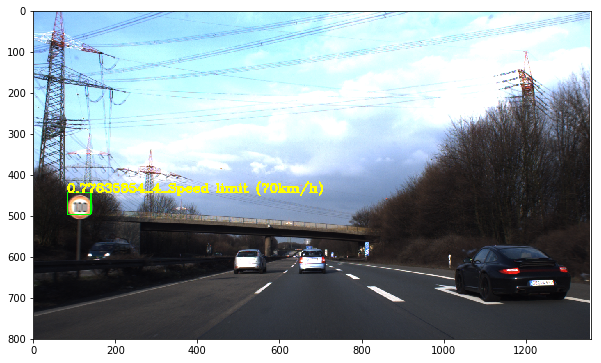
\includegraphics[height=2in]{chap5/image/data_detect/result/d_err1.png}}
    \subfloat[]
     {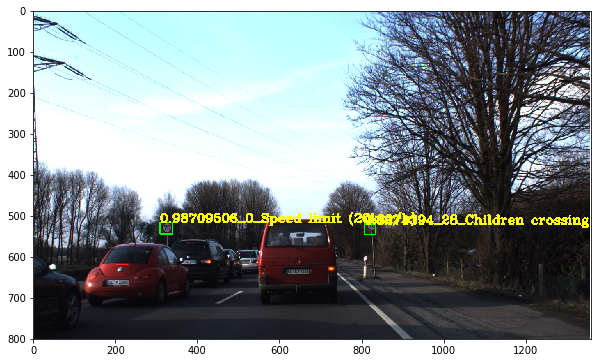
\includegraphics[height=2in]{chap5/image/data_detect/result/d_err2.png}}
\caption{Kết quả nhận diện không đúng}
\end{figure}
\section{Môi trường}
Ở đây tôi xin các công cụ và thư viện hỗ trợ được sử dụng cho khóa luận này.\\ \par
\textbf{Thiết bị}: Máy tính Dell Precision 7710, chip Core i7-6920HQ và cạc màn hình Quadro® M4000M.\\ \par
\textbf{Công nghệ}:
\hspace{5mm}
\begin{itemize}
\item[-]Ngôn ngữ lập trình: python
\item[-]Thư viện hỗ trợ: numpy, opencv, matplotlib, tensorflow, drakflow, keras,...
\item[-]Google Colab
\end{itemize}


\chapter{Kết Luận Và Hướng Phát Triển}
Kết quả của bài toán nhận diện biển báo vẫn chưa được chính xác do dữ liệu còn ít, vì vậy cần tìm cách tăng cường dữ liệu và tạo ra các bounding boxes chính xác cho dữ liệu tăng cường. Để tăng tỉ lệ ta cũng có thể thử nghiệm kết hợp nhiều mô hình khác nhau để các đặc trưng trích xuất ra chính xác, tổng quát nhất. Tuy nhiên, do điều kiện về thiết bị vật lý không cho phép tại thời điểm hiện tại nên tôi sẽ thử nghiệm, phát triển tiếp trong tương lai. \par
Như vậy qua bài toán nhận diện biển báo giao thông, tôi đã biết được cách hoạt động cũng như nguyên lý của học sâu trong các bài toán nhận diện. Tuy nhiên đó chỉ là một hạt cát trên sa mạc, với mỗi bài toán khác nhau sẽ có các vấn đề khác nhau và cần phải có các phương pháp tối ưu. Vì thế tôi sẽ tiếp tục nghiên cứu bài toán nhận diện để có thể phát triển các các bài toán ứng dụng thực tiễn ở Việt Nam như phát hiện vi phạm giao thông thông qua camera giao thông, nhận diện khuôn mặt để ứng dụng cho các ngôi nhà thông minh sau này. Không những thế bài toán nhận diện còn ứng dụng cho ngành y sinh, giúp bác sĩ có thể phát hiện được các khối u ở giai đoạn đầu mà mắt thường khó phát hiện.